\documentclass[twoside]{book}

% Packages required by doxygen
\usepackage{fixltx2e}
\usepackage{calc}
\usepackage{doxygen}
\usepackage[export]{adjustbox} % also loads graphicx
\usepackage{graphicx}
\usepackage[utf8]{inputenc}
\usepackage{makeidx}
\usepackage{multicol}
\usepackage{multirow}
\PassOptionsToPackage{warn}{textcomp}
\usepackage{textcomp}
\usepackage[nointegrals]{wasysym}
\usepackage[table]{xcolor}

% Font selection
\usepackage[T1]{fontenc}
\usepackage[scaled=.90]{helvet}
\usepackage{courier}
\usepackage{amssymb}
\usepackage{sectsty}
\renewcommand{\familydefault}{\sfdefault}
\allsectionsfont{%
  \fontseries{bc}\selectfont%
  \color{darkgray}%
}
\renewcommand{\DoxyLabelFont}{%
  \fontseries{bc}\selectfont%
  \color{darkgray}%
}
\newcommand{\+}{\discretionary{\mbox{\scriptsize$\hookleftarrow$}}{}{}}

% Page & text layout
\usepackage{geometry}
\geometry{%
  a4paper,%
  top=2.5cm,%
  bottom=2.5cm,%
  left=2.5cm,%
  right=2.5cm%
}
\tolerance=750
\hfuzz=15pt
\hbadness=750
\setlength{\emergencystretch}{15pt}
\setlength{\parindent}{0cm}
\setlength{\parskip}{3ex plus 2ex minus 2ex}
\makeatletter
\renewcommand{\paragraph}{%
  \@startsection{paragraph}{4}{0ex}{-1.0ex}{1.0ex}{%
    \normalfont\normalsize\bfseries\SS@parafont%
  }%
}
\renewcommand{\subparagraph}{%
  \@startsection{subparagraph}{5}{0ex}{-1.0ex}{1.0ex}{%
    \normalfont\normalsize\bfseries\SS@subparafont%
  }%
}
\makeatother

% Headers & footers
\usepackage{fancyhdr}
\pagestyle{fancyplain}
\fancyhead[LE]{\fancyplain{}{\bfseries\thepage}}
\fancyhead[CE]{\fancyplain{}{}}
\fancyhead[RE]{\fancyplain{}{\bfseries\leftmark}}
\fancyhead[LO]{\fancyplain{}{\bfseries\rightmark}}
\fancyhead[CO]{\fancyplain{}{}}
\fancyhead[RO]{\fancyplain{}{\bfseries\thepage}}
\fancyfoot[LE]{\fancyplain{}{}}
\fancyfoot[CE]{\fancyplain{}{}}
\fancyfoot[RE]{\fancyplain{}{\bfseries\scriptsize Generated by Doxygen }}
\fancyfoot[LO]{\fancyplain{}{\bfseries\scriptsize Generated by Doxygen }}
\fancyfoot[CO]{\fancyplain{}{}}
\fancyfoot[RO]{\fancyplain{}{}}
\renewcommand{\footrulewidth}{0.4pt}
\renewcommand{\chaptermark}[1]{%
  \markboth{#1}{}%
}
\renewcommand{\sectionmark}[1]{%
  \markright{\thesection\ #1}%
}

% Indices & bibliography
\usepackage{natbib}
\usepackage[titles]{tocloft}
\setcounter{tocdepth}{3}
\setcounter{secnumdepth}{5}
\makeindex

% Hyperlinks (required, but should be loaded last)
\usepackage{ifpdf}
\ifpdf
  \usepackage[pdftex,pagebackref=true]{hyperref}
\else
  \usepackage[ps2pdf,pagebackref=true]{hyperref}
\fi
\hypersetup{%
  colorlinks=true,%
  linkcolor=blue,%
  citecolor=blue,%
  unicode%
}

% Custom commands
\newcommand{\clearemptydoublepage}{%
  \newpage{\pagestyle{empty}\cleardoublepage}%
}

\usepackage{caption}
\captionsetup{labelsep=space,justification=centering,font={bf},singlelinecheck=off,skip=4pt,position=top}

%===== C O N T E N T S =====

\begin{document}

% Titlepage & ToC
\hypersetup{pageanchor=false,
             bookmarksnumbered=true,
             pdfencoding=unicode
            }
\pagenumbering{alph}
\begin{titlepage}
\vspace*{7cm}
\begin{center}%
{\Large Snake }\\
\vspace*{1cm}
{\large Generated by Doxygen 1.8.13}\\
\end{center}
\end{titlepage}
\clearemptydoublepage
\pagenumbering{roman}
\tableofcontents
\clearemptydoublepage
\pagenumbering{arabic}
\hypersetup{pageanchor=true}

%--- Begin generated contents ---
\chapter{Hierarchical Index}
\section{Class Hierarchy}
This inheritance list is sorted roughly, but not completely, alphabetically\+:\begin{DoxyCompactList}
\item \contentsline{section}{Board}{\pageref{class_board}}{}
\item \contentsline{section}{Chili\+Exception}{\pageref{class_chili_exception}}{}
\begin{DoxyCompactList}
\item \contentsline{section}{Graphics\+:\+:Exception}{\pageref{class_graphics_1_1_exception}}{}
\item \contentsline{section}{Main\+Window\+:\+:Exception}{\pageref{class_main_window_1_1_exception}}{}
\end{DoxyCompactList}
\item \contentsline{section}{Color}{\pageref{class_color}}{}
\item \contentsline{section}{Keyboard\+:\+:Event}{\pageref{class_keyboard_1_1_event}}{}
\item \contentsline{section}{Mouse\+:\+:Event}{\pageref{class_mouse_1_1_event}}{}
\item \contentsline{section}{Food}{\pageref{class_food}}{}
\item \contentsline{section}{Game}{\pageref{class_game}}{}
\item \contentsline{section}{Graphics}{\pageref{class_graphics}}{}
\item \contentsline{section}{H\+W\+N\+D\+Key}{\pageref{class_h_w_n_d_key}}{}
\begin{DoxyCompactList}
\item \contentsline{section}{Main\+Window}{\pageref{class_main_window}}{}
\end{DoxyCompactList}
\item \contentsline{section}{Keyboard}{\pageref{class_keyboard}}{}
\item \contentsline{section}{Mouse}{\pageref{class_mouse}}{}
\item \contentsline{section}{Pixel\+Location}{\pageref{class_pixel_location}}{}
\item \contentsline{section}{Snake}{\pageref{class_snake}}{}
\item \contentsline{section}{Sprite\+Codex}{\pageref{class_sprite_codex}}{}
\end{DoxyCompactList}

\chapter{Class Index}
\section{Class List}
Here are the classes, structs, unions and interfaces with brief descriptions\+:\begin{DoxyCompactList}
\item\contentsline{section}{\hyperlink{class_board}{Board} }{\pageref{class_board}}{}
\item\contentsline{section}{\hyperlink{class_chili_exception}{Chili\+Exception} }{\pageref{class_chili_exception}}{}
\item\contentsline{section}{\hyperlink{class_color}{Color} }{\pageref{class_color}}{}
\item\contentsline{section}{\hyperlink{class_keyboard_1_1_event}{Keyboard\+::\+Event} }{\pageref{class_keyboard_1_1_event}}{}
\item\contentsline{section}{\hyperlink{class_mouse_1_1_event}{Mouse\+::\+Event} }{\pageref{class_mouse_1_1_event}}{}
\item\contentsline{section}{\hyperlink{class_main_window_1_1_exception}{Main\+Window\+::\+Exception} }{\pageref{class_main_window_1_1_exception}}{}
\item\contentsline{section}{\hyperlink{class_graphics_1_1_exception}{Graphics\+::\+Exception} }{\pageref{class_graphics_1_1_exception}}{}
\item\contentsline{section}{\hyperlink{class_food}{Food} }{\pageref{class_food}}{}
\item\contentsline{section}{\hyperlink{class_game}{Game} }{\pageref{class_game}}{}
\item\contentsline{section}{\hyperlink{class_graphics}{Graphics} }{\pageref{class_graphics}}{}
\item\contentsline{section}{\hyperlink{class_h_w_n_d_key}{H\+W\+N\+D\+Key} }{\pageref{class_h_w_n_d_key}}{}
\item\contentsline{section}{\hyperlink{class_keyboard}{Keyboard} }{\pageref{class_keyboard}}{}
\item\contentsline{section}{\hyperlink{class_main_window}{Main\+Window} }{\pageref{class_main_window}}{}
\item\contentsline{section}{\hyperlink{class_mouse}{Mouse} }{\pageref{class_mouse}}{}
\item\contentsline{section}{\hyperlink{class_pixel_location}{Pixel\+Location} }{\pageref{class_pixel_location}}{}
\item\contentsline{section}{\hyperlink{class_snake}{Snake} }{\pageref{class_snake}}{}
\item\contentsline{section}{\hyperlink{class_sprite_codex}{Sprite\+Codex} }{\pageref{class_sprite_codex}}{}
\end{DoxyCompactList}

\chapter{Class Documentation}
\hypertarget{class_board}{}\section{Board Class Reference}
\label{class_board}\index{Board@{Board}}


{\ttfamily \#include $<$Board.\+h$>$}

\subsection*{Public Member Functions}
\begin{DoxyCompactItemize}
\item 
\hyperlink{class_board_a46374cb53089d5abbf7609234dca4828}{Board} (\hyperlink{class_graphics}{Graphics} \&gfx)
\item 
void \hyperlink{class_board_a3bfb1c528ae857f74b9ff3b3ba8d1911}{Draw\+Pixel} (const \hyperlink{class_pixel_location}{Pixel\+Location} \&loc)
\item 
void \hyperlink{class_board_a13216aad741156a095cf4509026a6649}{Draw\+Board} ()
\item 
bool \hyperlink{class_board_af00a708a0b6f2744b4494bd0d5fe0221}{is\+Inside\+Board} (const \hyperlink{class_pixel_location}{Pixel\+Location} loc) const
\end{DoxyCompactItemize}
\subsection*{Static Public Attributes}
\begin{DoxyCompactItemize}
\item 
\mbox{\Hypertarget{class_board_a492fe7c6d55d277f69dc67c2c08539ac}\label{class_board_a492fe7c6d55d277f69dc67c2c08539ac}} 
static constexpr int {\bfseries C\+E\+L\+L\+S\+\_\+X} = 20
\item 
\mbox{\Hypertarget{class_board_ad3b92faba492e95825f4018d41a0d977}\label{class_board_ad3b92faba492e95825f4018d41a0d977}} 
static constexpr int {\bfseries C\+E\+L\+L\+S\+\_\+Y} = 11
\item 
\mbox{\Hypertarget{class_board_ae512439f91443ec636ea6633a72ada06}\label{class_board_ae512439f91443ec636ea6633a72ada06}} 
static constexpr int {\bfseries S\+C\+R\+E\+E\+N\+\_\+\+W\+I\+D\+TH} = Graphics\+::\+Screen\+Width
\item 
\mbox{\Hypertarget{class_board_acdf9873415951e78df3fbae321381fd5}\label{class_board_acdf9873415951e78df3fbae321381fd5}} 
static constexpr int {\bfseries S\+C\+R\+E\+E\+N\+\_\+\+H\+E\+I\+G\+HT} = Graphics\+::\+Screen\+Height
\item 
\mbox{\Hypertarget{class_board_a01a6846968fd31e332f19e1978f27e0d}\label{class_board_a01a6846968fd31e332f19e1978f27e0d}} 
static constexpr int {\bfseries C\+E\+L\+L\+\_\+\+S\+I\+ZE} = 3
\item 
\mbox{\Hypertarget{class_board_a51e465bda972205b4c2e1e3b0fab6732}\label{class_board_a51e465bda972205b4c2e1e3b0fab6732}} 
static constexpr int {\bfseries C\+E\+L\+L\+\_\+\+L\+A\+R\+G\+E\+\_\+\+P\+I\+X\+E\+L\+\_\+\+O\+F\+F\+S\+ET} = 1
\item 
\mbox{\Hypertarget{class_board_a6915825e595c8a98ee5d083212a4f4c8}\label{class_board_a6915825e595c8a98ee5d083212a4f4c8}} 
static constexpr int {\bfseries C\+E\+L\+L\+\_\+\+I\+N\+C\+\_\+\+O\+F\+F\+S\+ET} = C\+E\+L\+L\+\_\+\+S\+I\+ZE + C\+E\+L\+L\+\_\+\+L\+A\+R\+G\+E\+\_\+\+P\+I\+X\+E\+L\+\_\+\+O\+F\+F\+S\+ET
\item 
static constexpr int {\bfseries G\+R\+I\+D\+\_\+\+W\+I\+D\+TH}
\item 
static constexpr int {\bfseries G\+R\+I\+D\+\_\+\+H\+E\+I\+G\+HT}
\item 
\mbox{\Hypertarget{class_board_a619774ab886154a3d5a74cf98ac42c69}\label{class_board_a619774ab886154a3d5a74cf98ac42c69}} 
static constexpr int {\bfseries L\+A\+R\+G\+E\+\_\+\+P\+I\+X\+E\+L\+\_\+\+D\+I\+M\+E\+N\+S\+I\+ON} = S\+C\+R\+E\+E\+N\+\_\+\+W\+I\+D\+TH / G\+R\+I\+D\+\_\+\+W\+I\+D\+TH
\item 
\mbox{\Hypertarget{class_board_ae9697a8aec0c7287651f758590e286c2}\label{class_board_ae9697a8aec0c7287651f758590e286c2}} 
static constexpr int {\bfseries L\+A\+R\+G\+E\+\_\+\+P\+I\+X\+E\+L\+\_\+\+O\+F\+F\+S\+ET} = 2
\item 
\mbox{\Hypertarget{class_board_a40ede8b5ef707e33c5e5423376ba0680}\label{class_board_a40ede8b5ef707e33c5e5423376ba0680}} 
static constexpr int {\bfseries unused\+PixelsX} = S\+C\+R\+E\+E\+N\+\_\+\+W\+I\+D\+TH -\/ (L\+A\+R\+G\+E\+\_\+\+P\+I\+X\+E\+L\+\_\+\+D\+I\+M\+E\+N\+S\+I\+ON) $\ast$ G\+R\+I\+D\+\_\+\+W\+I\+D\+TH
\item 
\mbox{\Hypertarget{class_board_a4e101f3a2d9dc6f1b001bb7764d58ff7}\label{class_board_a4e101f3a2d9dc6f1b001bb7764d58ff7}} 
static constexpr int {\bfseries unused\+PixelsY} = S\+C\+R\+E\+E\+N\+\_\+\+H\+E\+I\+G\+HT -\/ (L\+A\+R\+G\+E\+\_\+\+P\+I\+X\+E\+L\+\_\+\+D\+I\+M\+E\+N\+S\+I\+ON) $\ast$ G\+R\+I\+D\+\_\+\+H\+E\+I\+G\+HT
\end{DoxyCompactItemize}


\subsection{Detailed Description}
Manages the gaming board

\begin{DoxyAuthor}{Author}
\+: Benjamin Korady 
\end{DoxyAuthor}
\begin{DoxyVersion}{Version}
\+: 1.\+0 11/02/2017 
\end{DoxyVersion}


\subsection{Constructor \& Destructor Documentation}
\mbox{\Hypertarget{class_board_a46374cb53089d5abbf7609234dca4828}\label{class_board_a46374cb53089d5abbf7609234dca4828}} 
\index{Board@{Board}!Board@{Board}}
\index{Board@{Board}!Board@{Board}}
\subsubsection{\texorpdfstring{Board()}{Board()}}
{\footnotesize\ttfamily Board\+::\+Board (\begin{DoxyParamCaption}\item[{\hyperlink{class_graphics}{Graphics} \&}]{gfx }\end{DoxyParamCaption})}

Constructs a game board object Initializes background color to light green and pixel color to dark green / black


\begin{DoxyParams}{Parameters}
{\em gfx} & \hyperlink{class_graphics}{Graphics} processor reference \\
\hline
\end{DoxyParams}


\subsection{Member Function Documentation}
\mbox{\Hypertarget{class_board_a13216aad741156a095cf4509026a6649}\label{class_board_a13216aad741156a095cf4509026a6649}} 
\index{Board@{Board}!Draw\+Board@{Draw\+Board}}
\index{Draw\+Board@{Draw\+Board}!Board@{Board}}
\subsubsection{\texorpdfstring{Draw\+Board()}{DrawBoard()}}
{\footnotesize\ttfamily void Board\+::\+Draw\+Board (\begin{DoxyParamCaption}{ }\end{DoxyParamCaption})}

Draws the game board and background fill \mbox{\Hypertarget{class_board_a3bfb1c528ae857f74b9ff3b3ba8d1911}\label{class_board_a3bfb1c528ae857f74b9ff3b3ba8d1911}} 
\index{Board@{Board}!Draw\+Pixel@{Draw\+Pixel}}
\index{Draw\+Pixel@{Draw\+Pixel}!Board@{Board}}
\subsubsection{\texorpdfstring{Draw\+Pixel()}{DrawPixel()}}
{\footnotesize\ttfamily void Board\+::\+Draw\+Pixel (\begin{DoxyParamCaption}\item[{const \hyperlink{class_pixel_location}{Pixel\+Location} \&}]{loc }\end{DoxyParamCaption})}

Draws a large pixel to the screen (9 pc monitor pixels = 1 phone screen pixel) \href{http://i.imgur.com/RkFVcAk.png}{\tt http\+://i.\+imgur.\+com/\+Rk\+F\+Vc\+Ak.\+png}


\begin{DoxyParams}{Parameters}
{\em loc} & The location on the screen where the pixel is to be drawn \\
\hline
\end{DoxyParams}
\mbox{\Hypertarget{class_board_af00a708a0b6f2744b4494bd0d5fe0221}\label{class_board_af00a708a0b6f2744b4494bd0d5fe0221}} 
\index{Board@{Board}!is\+Inside\+Board@{is\+Inside\+Board}}
\index{is\+Inside\+Board@{is\+Inside\+Board}!Board@{Board}}
\subsubsection{\texorpdfstring{is\+Inside\+Board()}{isInsideBoard()}}
{\footnotesize\ttfamily bool Board\+::is\+Inside\+Board (\begin{DoxyParamCaption}\item[{const \hyperlink{class_pixel_location}{Pixel\+Location}}]{loc }\end{DoxyParamCaption}) const}

Checks if input location is inside the game board


\begin{DoxyParams}{Parameters}
{\em loc} & The input location to check against the game board \\
\hline
\end{DoxyParams}
\begin{DoxyReturn}{Returns}
bool 
\end{DoxyReturn}


\subsection{Member Data Documentation}
\mbox{\Hypertarget{class_board_aff34c4b148c4ea0ee9fe7254a529ceee}\label{class_board_aff34c4b148c4ea0ee9fe7254a529ceee}} 
\index{Board@{Board}!G\+R\+I\+D\+\_\+\+H\+E\+I\+G\+HT@{G\+R\+I\+D\+\_\+\+H\+E\+I\+G\+HT}}
\index{G\+R\+I\+D\+\_\+\+H\+E\+I\+G\+HT@{G\+R\+I\+D\+\_\+\+H\+E\+I\+G\+HT}!Board@{Board}}
\subsubsection{\texorpdfstring{G\+R\+I\+D\+\_\+\+H\+E\+I\+G\+HT}{GRID\_HEIGHT}}
{\footnotesize\ttfamily constexpr int Board\+::\+G\+R\+I\+D\+\_\+\+H\+E\+I\+G\+HT\hspace{0.3cm}{\ttfamily [static]}}

{\bfseries Initial value\+:}
\begin{DoxyCode}
= CELLS\_Y * CELL\_SIZE + (CELLS\_Y - 1) * CELL\_LARGE\_PIXEL\_OFFSET + 2 * CELL\_LARGE\_PIXEL\_OFFSET
                                       + 2 * CELL\_LARGE\_PIXEL\_OFFSET
\end{DoxyCode}
\mbox{\Hypertarget{class_board_ae781948bea97fe9c0469b10b0f61bf7d}\label{class_board_ae781948bea97fe9c0469b10b0f61bf7d}} 
\index{Board@{Board}!G\+R\+I\+D\+\_\+\+W\+I\+D\+TH@{G\+R\+I\+D\+\_\+\+W\+I\+D\+TH}}
\index{G\+R\+I\+D\+\_\+\+W\+I\+D\+TH@{G\+R\+I\+D\+\_\+\+W\+I\+D\+TH}!Board@{Board}}
\subsubsection{\texorpdfstring{G\+R\+I\+D\+\_\+\+W\+I\+D\+TH}{GRID\_WIDTH}}
{\footnotesize\ttfamily constexpr int Board\+::\+G\+R\+I\+D\+\_\+\+W\+I\+D\+TH\hspace{0.3cm}{\ttfamily [static]}}

{\bfseries Initial value\+:}
\begin{DoxyCode}
= CELLS\_X * CELL\_SIZE + (CELLS\_X-1) * CELL\_LARGE\_PIXEL\_OFFSET + 2 * CELL\_LARGE\_PIXEL\_OFFSET
                                      + 2 * CELL\_LARGE\_PIXEL\_OFFSET
\end{DoxyCode}


The documentation for this class was generated from the following files\+:\begin{DoxyCompactItemize}
\item 
Board.\+h\item 
Board.\+cpp\end{DoxyCompactItemize}

\hypertarget{class_chili_exception}{}\section{Chili\+Exception Class Reference}
\label{class_chili_exception}\index{Chili\+Exception@{Chili\+Exception}}
Inheritance diagram for Chili\+Exception\+:\begin{figure}[H]
\begin{center}
\leavevmode
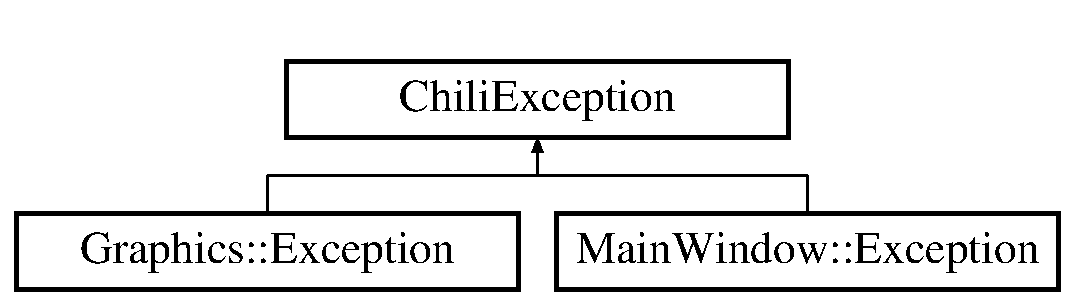
\includegraphics[height=2.000000cm]{class_chili_exception}
\end{center}
\end{figure}
\subsection*{Public Member Functions}
\begin{DoxyCompactItemize}
\item 
\mbox{\Hypertarget{class_chili_exception_ab08ab747307f2a3116b61d8c56e6287b}\label{class_chili_exception_ab08ab747307f2a3116b61d8c56e6287b}} 
{\bfseries Chili\+Exception} (const wchar\+\_\+t $\ast$file, unsigned int line, const std\+::wstring \&note=L\char`\"{}\char`\"{})
\item 
\mbox{\Hypertarget{class_chili_exception_ac91c28909ddc75b51afeef77f971fda6}\label{class_chili_exception_ac91c28909ddc75b51afeef77f971fda6}} 
const std\+::wstring \& {\bfseries Get\+Note} () const
\item 
\mbox{\Hypertarget{class_chili_exception_a6ec0a02f643f907e01df8c297f0e52bf}\label{class_chili_exception_a6ec0a02f643f907e01df8c297f0e52bf}} 
const std\+::wstring \& {\bfseries Get\+File} () const
\item 
\mbox{\Hypertarget{class_chili_exception_a0acc5bd63c23bee4354ddcea9be2e7e1}\label{class_chili_exception_a0acc5bd63c23bee4354ddcea9be2e7e1}} 
unsigned int {\bfseries Get\+Line} () const
\item 
\mbox{\Hypertarget{class_chili_exception_ab871cd7426216808049fd7fb4c4413e0}\label{class_chili_exception_ab871cd7426216808049fd7fb4c4413e0}} 
std\+::wstring {\bfseries Get\+Location} () const
\item 
\mbox{\Hypertarget{class_chili_exception_a1d3f4e1c02fa769c64f8d3439b60436f}\label{class_chili_exception_a1d3f4e1c02fa769c64f8d3439b60436f}} 
virtual std\+::wstring {\bfseries Get\+Full\+Message} () const =0
\item 
\mbox{\Hypertarget{class_chili_exception_adc6a2ae915cdb20d5a161cdc78f43f9b}\label{class_chili_exception_adc6a2ae915cdb20d5a161cdc78f43f9b}} 
virtual std\+::wstring {\bfseries Get\+Exception\+Type} () const =0
\end{DoxyCompactItemize}


The documentation for this class was generated from the following file\+:\begin{DoxyCompactItemize}
\item 
Chili\+Exception.\+h\end{DoxyCompactItemize}

\hypertarget{class_color}{}\section{Color Class Reference}
\label{class_color}\index{Color@{Color}}
\subsection*{Public Member Functions}
\begin{DoxyCompactItemize}
\item 
\mbox{\Hypertarget{class_color_aee4ab42a1616f7e0639c6cb1daa30d64}\label{class_color_aee4ab42a1616f7e0639c6cb1daa30d64}} 
constexpr {\bfseries Color} (const \hyperlink{class_color}{Color} \&col)
\item 
\mbox{\Hypertarget{class_color_ac354c51018de687c5f883c3bdad7d6cd}\label{class_color_ac354c51018de687c5f883c3bdad7d6cd}} 
constexpr {\bfseries Color} (unsigned int dw)
\item 
\mbox{\Hypertarget{class_color_aa8b0bda7bf46733f7daec168c6a209f6}\label{class_color_aa8b0bda7bf46733f7daec168c6a209f6}} 
constexpr {\bfseries Color} (unsigned char x, unsigned char r, unsigned char g, unsigned char b)
\item 
\mbox{\Hypertarget{class_color_a38a4c8384e3231bc106a9d70004e1701}\label{class_color_a38a4c8384e3231bc106a9d70004e1701}} 
constexpr {\bfseries Color} (unsigned char r, unsigned char g, unsigned char b)
\item 
\mbox{\Hypertarget{class_color_ae05c2cc6f91004653f8d2fb76c4fa727}\label{class_color_ae05c2cc6f91004653f8d2fb76c4fa727}} 
constexpr {\bfseries Color} (\hyperlink{class_color}{Color} col, unsigned char x)
\item 
\mbox{\Hypertarget{class_color_a2f9b3488c4c8b27b2f83649a297c50e7}\label{class_color_a2f9b3488c4c8b27b2f83649a297c50e7}} 
\hyperlink{class_color}{Color} \& {\bfseries operator=} (\hyperlink{class_color}{Color} color)
\item 
\mbox{\Hypertarget{class_color_a60370781fc2b718d79793b5a48e0f86a}\label{class_color_a60370781fc2b718d79793b5a48e0f86a}} 
constexpr unsigned char {\bfseries GetX} () const
\item 
\mbox{\Hypertarget{class_color_a196c393b4fd25f7a354555e68f102598}\label{class_color_a196c393b4fd25f7a354555e68f102598}} 
constexpr unsigned char {\bfseries GetA} () const
\item 
\mbox{\Hypertarget{class_color_a481e58f883a627ddfa9c8cdeb295891e}\label{class_color_a481e58f883a627ddfa9c8cdeb295891e}} 
constexpr unsigned char {\bfseries GetR} () const
\item 
\mbox{\Hypertarget{class_color_ab3d9b9a9ee6022dcad662ed9b0051ca9}\label{class_color_ab3d9b9a9ee6022dcad662ed9b0051ca9}} 
constexpr unsigned char {\bfseries GetG} () const
\item 
\mbox{\Hypertarget{class_color_a633c52d431432c9b8e5b3ff7dbf9d23a}\label{class_color_a633c52d431432c9b8e5b3ff7dbf9d23a}} 
constexpr unsigned char {\bfseries GetB} () const
\item 
\mbox{\Hypertarget{class_color_a96261574ca486337f4442be7916a070f}\label{class_color_a96261574ca486337f4442be7916a070f}} 
void {\bfseries SetX} (unsigned char x)
\item 
\mbox{\Hypertarget{class_color_a5b91faddcdde22a2af12c0de50a3f3fa}\label{class_color_a5b91faddcdde22a2af12c0de50a3f3fa}} 
void {\bfseries SetA} (unsigned char a)
\item 
\mbox{\Hypertarget{class_color_aa666f3043251a75e9365ea5bb725b78c}\label{class_color_aa666f3043251a75e9365ea5bb725b78c}} 
void {\bfseries SetR} (unsigned char r)
\item 
\mbox{\Hypertarget{class_color_a79b9dc911c6ff5d237786344d460aa67}\label{class_color_a79b9dc911c6ff5d237786344d460aa67}} 
void {\bfseries SetG} (unsigned char g)
\item 
\mbox{\Hypertarget{class_color_afb9bdd7639f6ed0ad2334a9ffc92653c}\label{class_color_afb9bdd7639f6ed0ad2334a9ffc92653c}} 
void {\bfseries SetB} (unsigned char b)
\end{DoxyCompactItemize}
\subsection*{Public Attributes}
\begin{DoxyCompactItemize}
\item 
\mbox{\Hypertarget{class_color_ad467ce2d3ab71b51ec245ef4a64967ef}\label{class_color_ad467ce2d3ab71b51ec245ef4a64967ef}} 
unsigned int {\bfseries dword}
\end{DoxyCompactItemize}


The documentation for this class was generated from the following file\+:\begin{DoxyCompactItemize}
\item 
Colors.\+h\end{DoxyCompactItemize}

\hypertarget{class_keyboard_1_1_event}{}\section{Keyboard\+:\+:Event Class Reference}
\label{class_keyboard_1_1_event}\index{Keyboard\+::\+Event@{Keyboard\+::\+Event}}
\subsection*{Public Types}
\begin{DoxyCompactItemize}
\item 
\mbox{\Hypertarget{class_keyboard_1_1_event_aaa12f942b71b42761c3bec96f3a67075}\label{class_keyboard_1_1_event_aaa12f942b71b42761c3bec96f3a67075}} 
enum {\bfseries Type} \{ {\bfseries Press}, 
{\bfseries Release}, 
{\bfseries Invalid}
 \}
\end{DoxyCompactItemize}
\subsection*{Public Member Functions}
\begin{DoxyCompactItemize}
\item 
\mbox{\Hypertarget{class_keyboard_1_1_event_abf5090b40bbd93c32878521ae61de3b7}\label{class_keyboard_1_1_event_abf5090b40bbd93c32878521ae61de3b7}} 
{\bfseries Event} (Type type, unsigned char code)
\item 
\mbox{\Hypertarget{class_keyboard_1_1_event_ae789b12e35794b03858e0decd61dda71}\label{class_keyboard_1_1_event_ae789b12e35794b03858e0decd61dda71}} 
bool {\bfseries Is\+Press} () const
\item 
\mbox{\Hypertarget{class_keyboard_1_1_event_a23b254195a1305b536efecea4c5ecb4b}\label{class_keyboard_1_1_event_a23b254195a1305b536efecea4c5ecb4b}} 
bool {\bfseries Is\+Release} () const
\item 
\mbox{\Hypertarget{class_keyboard_1_1_event_a5b7cea14f9a1f56e630d538ab4cbc1b7}\label{class_keyboard_1_1_event_a5b7cea14f9a1f56e630d538ab4cbc1b7}} 
bool {\bfseries Is\+Valid} () const
\item 
\mbox{\Hypertarget{class_keyboard_1_1_event_a00b59fcaaf7537e511a7d9eaa88b78c4}\label{class_keyboard_1_1_event_a00b59fcaaf7537e511a7d9eaa88b78c4}} 
unsigned char {\bfseries Get\+Code} () const
\end{DoxyCompactItemize}


The documentation for this class was generated from the following file\+:\begin{DoxyCompactItemize}
\item 
Keyboard.\+h\end{DoxyCompactItemize}

\hypertarget{class_mouse_1_1_event}{}\section{Mouse\+:\+:Event Class Reference}
\label{class_mouse_1_1_event}\index{Mouse\+::\+Event@{Mouse\+::\+Event}}
\subsection*{Public Types}
\begin{DoxyCompactItemize}
\item 
\mbox{\Hypertarget{class_mouse_1_1_event_a32491602b4d05d2c0602db8e1e01686f}\label{class_mouse_1_1_event_a32491602b4d05d2c0602db8e1e01686f}} 
enum {\bfseries Type} \{ \newline
{\bfseries L\+Press}, 
{\bfseries L\+Release}, 
{\bfseries R\+Press}, 
{\bfseries R\+Release}, 
\newline
{\bfseries Wheel\+Up}, 
{\bfseries Wheel\+Down}, 
{\bfseries Move}, 
{\bfseries Invalid}
 \}
\end{DoxyCompactItemize}
\subsection*{Public Member Functions}
\begin{DoxyCompactItemize}
\item 
\mbox{\Hypertarget{class_mouse_1_1_event_aea4f1facdefa1854fe3c72d4902b0bee}\label{class_mouse_1_1_event_aea4f1facdefa1854fe3c72d4902b0bee}} 
{\bfseries Event} (Type type, const \hyperlink{class_mouse}{Mouse} \&parent)
\item 
\mbox{\Hypertarget{class_mouse_1_1_event_af11f64f339135a49c06c174a8fd2e3dc}\label{class_mouse_1_1_event_af11f64f339135a49c06c174a8fd2e3dc}} 
bool {\bfseries Is\+Valid} () const
\item 
\mbox{\Hypertarget{class_mouse_1_1_event_a3f75592ce8c5bf94d5404f17df3784f8}\label{class_mouse_1_1_event_a3f75592ce8c5bf94d5404f17df3784f8}} 
Type {\bfseries Get\+Type} () const
\item 
\mbox{\Hypertarget{class_mouse_1_1_event_a9e6754c38abf6dc80c77a6fc5d4539b5}\label{class_mouse_1_1_event_a9e6754c38abf6dc80c77a6fc5d4539b5}} 
std\+::pair$<$ int, int $>$ {\bfseries Get\+Pos} () const
\item 
\mbox{\Hypertarget{class_mouse_1_1_event_a863eb1934b554fb081c90c9b1b28b4d6}\label{class_mouse_1_1_event_a863eb1934b554fb081c90c9b1b28b4d6}} 
int {\bfseries Get\+PosX} () const
\item 
\mbox{\Hypertarget{class_mouse_1_1_event_a85460659bdc08b0e1fe9bcd6d4c7d0a3}\label{class_mouse_1_1_event_a85460659bdc08b0e1fe9bcd6d4c7d0a3}} 
int {\bfseries Get\+PosY} () const
\item 
\mbox{\Hypertarget{class_mouse_1_1_event_aa03f692d57d82f23f9e2fb7cbeb508d2}\label{class_mouse_1_1_event_aa03f692d57d82f23f9e2fb7cbeb508d2}} 
bool {\bfseries Left\+Is\+Pressed} () const
\item 
\mbox{\Hypertarget{class_mouse_1_1_event_ab7a5f5d163e0d59141d23ddc8469d94e}\label{class_mouse_1_1_event_ab7a5f5d163e0d59141d23ddc8469d94e}} 
bool {\bfseries Right\+Is\+Pressed} () const
\end{DoxyCompactItemize}


The documentation for this class was generated from the following file\+:\begin{DoxyCompactItemize}
\item 
Mouse.\+h\end{DoxyCompactItemize}

\hypertarget{class_main_window_1_1_exception}{}\section{Main\+Window\+:\+:Exception Class Reference}
\label{class_main_window_1_1_exception}\index{Main\+Window\+::\+Exception@{Main\+Window\+::\+Exception}}
Inheritance diagram for Main\+Window\+:\+:Exception\+:\begin{figure}[H]
\begin{center}
\leavevmode
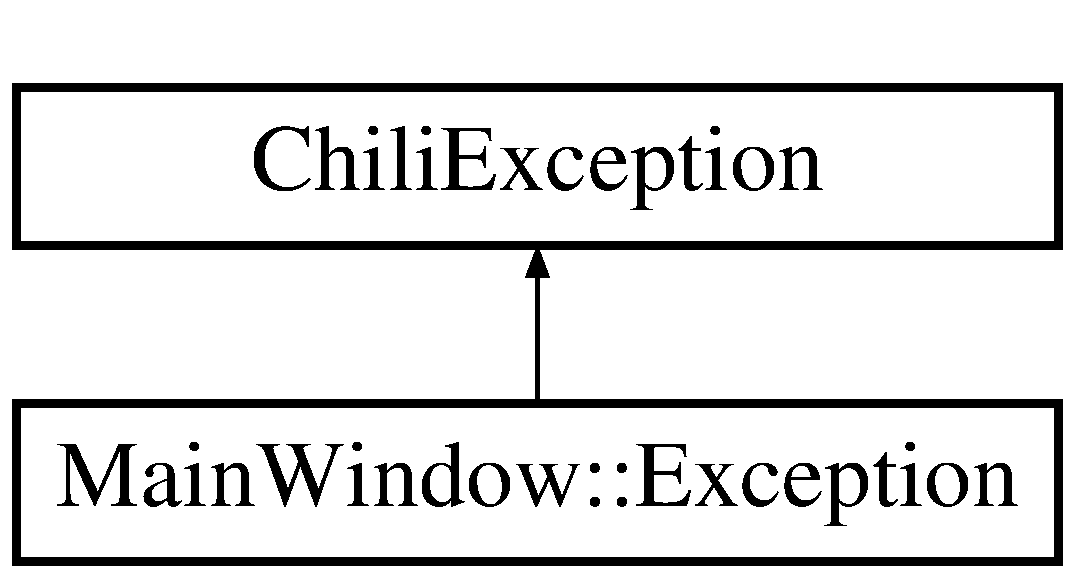
\includegraphics[height=2.000000cm]{class_main_window_1_1_exception}
\end{center}
\end{figure}
\subsection*{Public Member Functions}
\begin{DoxyCompactItemize}
\item 
\mbox{\Hypertarget{class_main_window_1_1_exception_ac18eb476a16e0e98803d385c7097d6e0}\label{class_main_window_1_1_exception_ac18eb476a16e0e98803d385c7097d6e0}} 
virtual std\+::wstring {\bfseries Get\+Full\+Message} () const override
\item 
\mbox{\Hypertarget{class_main_window_1_1_exception_a08e7ee28c3b282928f2c5de063a4bd83}\label{class_main_window_1_1_exception_a08e7ee28c3b282928f2c5de063a4bd83}} 
virtual std\+::wstring {\bfseries Get\+Exception\+Type} () const override
\end{DoxyCompactItemize}


The documentation for this class was generated from the following file\+:\begin{DoxyCompactItemize}
\item 
Main\+Window.\+h\end{DoxyCompactItemize}

\hypertarget{class_graphics_1_1_exception}{}\section{Graphics\+:\+:Exception Class Reference}
\label{class_graphics_1_1_exception}\index{Graphics\+::\+Exception@{Graphics\+::\+Exception}}
Inheritance diagram for Graphics\+:\+:Exception\+:\begin{figure}[H]
\begin{center}
\leavevmode
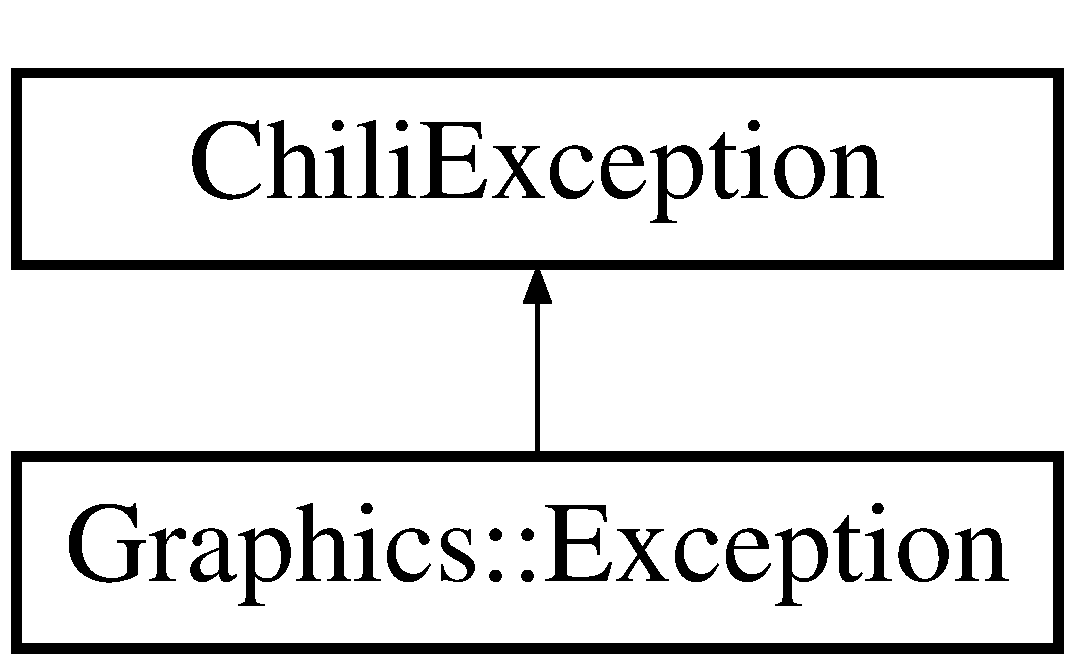
\includegraphics[height=2.000000cm]{class_graphics_1_1_exception}
\end{center}
\end{figure}
\subsection*{Public Member Functions}
\begin{DoxyCompactItemize}
\item 
\mbox{\Hypertarget{class_graphics_1_1_exception_a4b41b1546bc1cfed820ce788bb92be66}\label{class_graphics_1_1_exception_a4b41b1546bc1cfed820ce788bb92be66}} 
{\bfseries Exception} (H\+R\+E\+S\+U\+LT hr, const std\+::wstring \&note, const wchar\+\_\+t $\ast$file, unsigned int line)
\item 
\mbox{\Hypertarget{class_graphics_1_1_exception_ac17beac957a2bd74fd7057c0854cec2b}\label{class_graphics_1_1_exception_ac17beac957a2bd74fd7057c0854cec2b}} 
std\+::wstring {\bfseries Get\+Error\+Name} () const
\item 
\mbox{\Hypertarget{class_graphics_1_1_exception_a5c772df700d65afebeede2458517b79d}\label{class_graphics_1_1_exception_a5c772df700d65afebeede2458517b79d}} 
std\+::wstring {\bfseries Get\+Error\+Description} () const
\item 
\mbox{\Hypertarget{class_graphics_1_1_exception_a72385eeb123d5171055c501c52833563}\label{class_graphics_1_1_exception_a72385eeb123d5171055c501c52833563}} 
virtual std\+::wstring {\bfseries Get\+Full\+Message} () const override
\item 
\mbox{\Hypertarget{class_graphics_1_1_exception_ac8b78d9f50a178dc70407079a6958602}\label{class_graphics_1_1_exception_ac8b78d9f50a178dc70407079a6958602}} 
virtual std\+::wstring {\bfseries Get\+Exception\+Type} () const override
\end{DoxyCompactItemize}


The documentation for this class was generated from the following files\+:\begin{DoxyCompactItemize}
\item 
Graphics.\+h\item 
Graphics.\+cpp\end{DoxyCompactItemize}

\hypertarget{class_food}{}\section{Food Class Reference}
\label{class_food}\index{Food@{Food}}


{\ttfamily \#include $<$Food.\+h$>$}

\subsection*{Public Member Functions}
\begin{DoxyCompactItemize}
\item 
\hyperlink{class_food_a75d4d7f76fd495cc8133302ca9fdc485}{Food} ()
\item 
\hyperlink{class_food_abf88eb6961b943a2d481c08eca91cc2d}{Food} (\hyperlink{class_pixel_location}{Pixel\+Location} loc)
\item 
void \hyperlink{class_food_a2757ddcb688ca74d3e2e79d645e0ed0e}{draw} (\hyperlink{class_board}{Board} \&brd) const
\item 
\hyperlink{class_pixel_location}{Pixel\+Location} \hyperlink{class_food_a7c3ffe081ee2b479696c0c89ed95455c}{get\+Location} () const
\item 
void \hyperlink{class_food_afcd8485cf59e61adcc28cfc237bf3001}{respawn} (const \hyperlink{class_snake}{Snake} \&snek)
\end{DoxyCompactItemize}


\subsection{Detailed Description}
Manages the food object

\begin{DoxyAuthor}{Author}
\+: Benjamin Korady 
\end{DoxyAuthor}
\begin{DoxyVersion}{Version}
\+: 1.\+0 11/02/2017 
\end{DoxyVersion}


\subsection{Constructor \& Destructor Documentation}
\mbox{\Hypertarget{class_food_a75d4d7f76fd495cc8133302ca9fdc485}\label{class_food_a75d4d7f76fd495cc8133302ca9fdc485}} 
\index{Food@{Food}!Food@{Food}}
\index{Food@{Food}!Food@{Food}}
\subsubsection{\texorpdfstring{Food()}{Food()}\hspace{0.1cm}{\footnotesize\ttfamily [1/2]}}
{\footnotesize\ttfamily Food\+::\+Food (\begin{DoxyParamCaption}{ }\end{DoxyParamCaption})}

Constructs food object at the center of the screen \mbox{\Hypertarget{class_food_abf88eb6961b943a2d481c08eca91cc2d}\label{class_food_abf88eb6961b943a2d481c08eca91cc2d}} 
\index{Food@{Food}!Food@{Food}}
\index{Food@{Food}!Food@{Food}}
\subsubsection{\texorpdfstring{Food()}{Food()}\hspace{0.1cm}{\footnotesize\ttfamily [2/2]}}
{\footnotesize\ttfamily Food\+::\+Food (\begin{DoxyParamCaption}\item[{\hyperlink{class_pixel_location}{Pixel\+Location}}]{loc }\end{DoxyParamCaption})}

Constructs food object at the input location


\begin{DoxyParams}{Parameters}
{\em loc} & Specifies the location where the object is to be created \\
\hline
\end{DoxyParams}


\subsection{Member Function Documentation}
\mbox{\Hypertarget{class_food_a2757ddcb688ca74d3e2e79d645e0ed0e}\label{class_food_a2757ddcb688ca74d3e2e79d645e0ed0e}} 
\index{Food@{Food}!draw@{draw}}
\index{draw@{draw}!Food@{Food}}
\subsubsection{\texorpdfstring{draw()}{draw()}}
{\footnotesize\ttfamily void Food\+::draw (\begin{DoxyParamCaption}\item[{\hyperlink{class_board}{Board} \&}]{brd }\end{DoxyParamCaption}) const}

Draws the food onto the board


\begin{DoxyParams}{Parameters}
{\em brd} & \hyperlink{class_board}{Board} object reference \\
\hline
\end{DoxyParams}
\mbox{\Hypertarget{class_food_a7c3ffe081ee2b479696c0c89ed95455c}\label{class_food_a7c3ffe081ee2b479696c0c89ed95455c}} 
\index{Food@{Food}!get\+Location@{get\+Location}}
\index{get\+Location@{get\+Location}!Food@{Food}}
\subsubsection{\texorpdfstring{get\+Location()}{getLocation()}}
{\footnotesize\ttfamily \hyperlink{class_pixel_location}{Pixel\+Location} Food\+::get\+Location (\begin{DoxyParamCaption}{ }\end{DoxyParamCaption}) const}

Returns the location of the food

\begin{DoxyReturn}{Returns}
loc 
\end{DoxyReturn}
\mbox{\Hypertarget{class_food_afcd8485cf59e61adcc28cfc237bf3001}\label{class_food_afcd8485cf59e61adcc28cfc237bf3001}} 
\index{Food@{Food}!respawn@{respawn}}
\index{respawn@{respawn}!Food@{Food}}
\subsubsection{\texorpdfstring{respawn()}{respawn()}}
{\footnotesize\ttfamily void Food\+::respawn (\begin{DoxyParamCaption}\item[{const \hyperlink{class_snake}{Snake} \&}]{snek }\end{DoxyParamCaption})}

Relocates the food at a random location on the board avoiding the snake\textquotesingle{}s body


\begin{DoxyParams}{Parameters}
{\em snek} & \hyperlink{class_snake}{Snake} object that needs to be avoided when placing food \\
\hline
\end{DoxyParams}


The documentation for this class was generated from the following files\+:\begin{DoxyCompactItemize}
\item 
Food.\+h\item 
Food.\+cpp\end{DoxyCompactItemize}

\hypertarget{class_game}{}\section{Game Class Reference}
\label{class_game}\index{Game@{Game}}
\subsection*{Public Member Functions}
\begin{DoxyCompactItemize}
\item 
\mbox{\Hypertarget{class_game_ac7d110c84639f35b32098bcc22966446}\label{class_game_ac7d110c84639f35b32098bcc22966446}} 
{\bfseries Game} (class \hyperlink{class_main_window}{Main\+Window} \&wnd)
\item 
\mbox{\Hypertarget{class_game_abb28875d74d25fa9e0dcdbe37c6ad89c}\label{class_game_abb28875d74d25fa9e0dcdbe37c6ad89c}} 
{\bfseries Game} (const \hyperlink{class_game}{Game} \&)=delete
\item 
\mbox{\Hypertarget{class_game_a4d0c0503733cc50b0b5cb8d7ef1237ec}\label{class_game_a4d0c0503733cc50b0b5cb8d7ef1237ec}} 
\hyperlink{class_game}{Game} \& {\bfseries operator=} (const \hyperlink{class_game}{Game} \&)=delete
\item 
\mbox{\Hypertarget{class_game_ac7f625a10c7d19d4d38a31f400c77ddc}\label{class_game_ac7f625a10c7d19d4d38a31f400c77ddc}} 
void {\bfseries Go} ()
\end{DoxyCompactItemize}


The documentation for this class was generated from the following files\+:\begin{DoxyCompactItemize}
\item 
Game.\+h\item 
Game.\+cpp\end{DoxyCompactItemize}

\hypertarget{class_graphics}{}\section{Graphics Class Reference}
\label{class_graphics}\index{Graphics@{Graphics}}
\subsection*{Classes}
\begin{DoxyCompactItemize}
\item 
class \hyperlink{class_graphics_1_1_exception}{Exception}
\end{DoxyCompactItemize}
\subsection*{Public Member Functions}
\begin{DoxyCompactItemize}
\item 
\mbox{\Hypertarget{class_graphics_ab29fadd0d25fa1313d89c84443f49122}\label{class_graphics_ab29fadd0d25fa1313d89c84443f49122}} 
{\bfseries Graphics} (class \hyperlink{class_h_w_n_d_key}{H\+W\+N\+D\+Key} \&key)
\item 
\mbox{\Hypertarget{class_graphics_abe2f13f24a1d35c55fdac10a282744eb}\label{class_graphics_abe2f13f24a1d35c55fdac10a282744eb}} 
{\bfseries Graphics} (const \hyperlink{class_graphics}{Graphics} \&)=delete
\item 
\mbox{\Hypertarget{class_graphics_abaf6bc20f9541026835dfee157ac5efb}\label{class_graphics_abaf6bc20f9541026835dfee157ac5efb}} 
\hyperlink{class_graphics}{Graphics} \& {\bfseries operator=} (const \hyperlink{class_graphics}{Graphics} \&)=delete
\item 
\mbox{\Hypertarget{class_graphics_a56203cba547bde8af2eadda01e0d17c3}\label{class_graphics_a56203cba547bde8af2eadda01e0d17c3}} 
void {\bfseries End\+Frame} ()
\item 
\mbox{\Hypertarget{class_graphics_ae9f5bcaa267fdff06bbfcf1e2ddf7137}\label{class_graphics_ae9f5bcaa267fdff06bbfcf1e2ddf7137}} 
void {\bfseries Begin\+Frame} ()
\item 
\mbox{\Hypertarget{class_graphics_a64e7971066ee21f5b77aa525742f29e2}\label{class_graphics_a64e7971066ee21f5b77aa525742f29e2}} 
void {\bfseries Put\+Pixel} (int x, int y, int r, int g, int b)
\item 
\mbox{\Hypertarget{class_graphics_a69fae0334426fd8a8a271d9843d4f7fe}\label{class_graphics_a69fae0334426fd8a8a271d9843d4f7fe}} 
void {\bfseries Put\+Pixel} (int x, int y, \hyperlink{class_color}{Color} c)
\item 
\mbox{\Hypertarget{class_graphics_ab90ddf2598eb05b8161e18683796188f}\label{class_graphics_ab90ddf2598eb05b8161e18683796188f}} 
void {\bfseries Draw\+Rect} (int x0, int y0, int x1, int y1, \hyperlink{class_color}{Color} c)
\item 
\mbox{\Hypertarget{class_graphics_a666082287b610f4928feddf666ee296d}\label{class_graphics_a666082287b610f4928feddf666ee296d}} 
void {\bfseries Draw\+Rect\+Dim} (int x0, int y0, int width, int height, \hyperlink{class_color}{Color} c)
\end{DoxyCompactItemize}
\subsection*{Static Public Attributes}
\begin{DoxyCompactItemize}
\item 
\mbox{\Hypertarget{class_graphics_ad9975c4111f24684740c6fedc3dc9659}\label{class_graphics_ad9975c4111f24684740c6fedc3dc9659}} 
static constexpr int {\bfseries Screen\+Width} = 800
\item 
\mbox{\Hypertarget{class_graphics_a315cf431c3f771beed8da6ce04955c9d}\label{class_graphics_a315cf431c3f771beed8da6ce04955c9d}} 
static constexpr int {\bfseries Screen\+Height} = 600
\end{DoxyCompactItemize}


The documentation for this class was generated from the following files\+:\begin{DoxyCompactItemize}
\item 
Graphics.\+h\item 
Graphics.\+cpp\end{DoxyCompactItemize}

\hypertarget{class_h_w_n_d_key}{}\section{H\+W\+N\+D\+Key Class Reference}
\label{class_h_w_n_d_key}\index{H\+W\+N\+D\+Key@{H\+W\+N\+D\+Key}}
Inheritance diagram for H\+W\+N\+D\+Key\+:\begin{figure}[H]
\begin{center}
\leavevmode
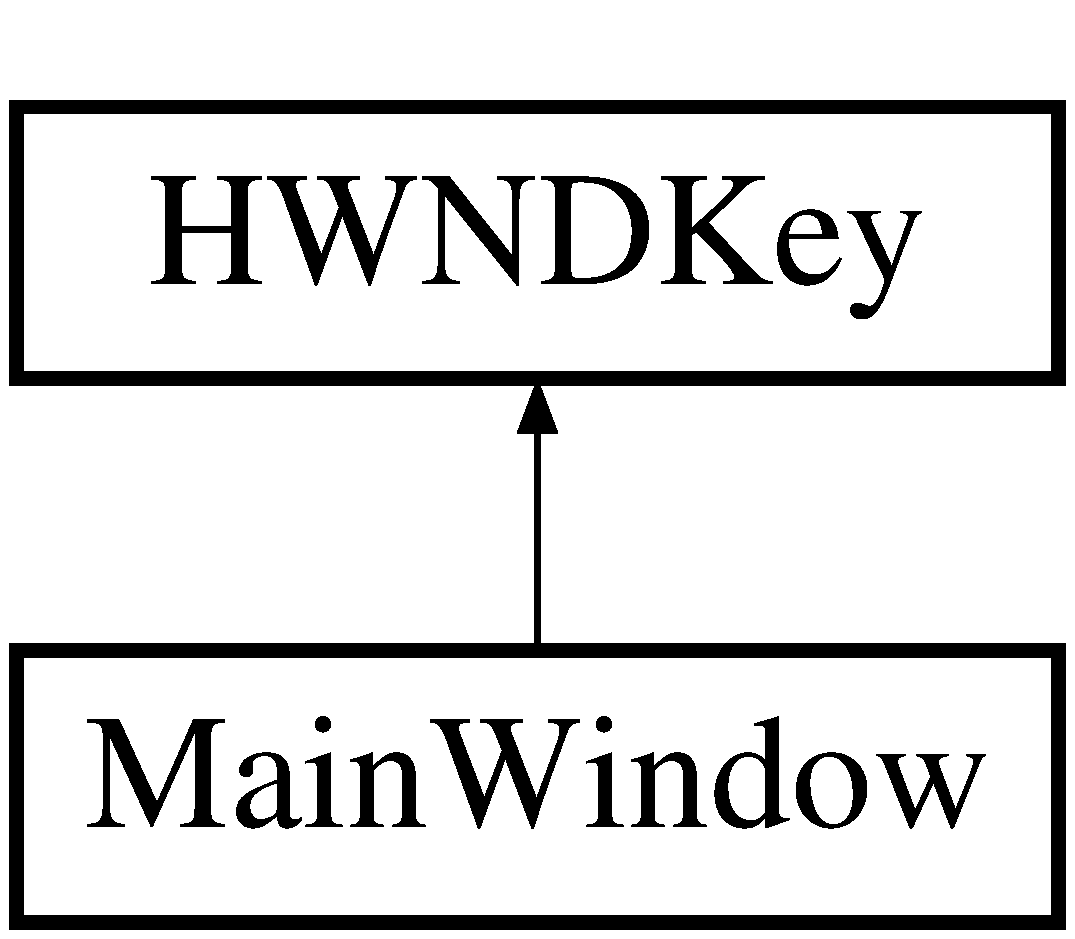
\includegraphics[height=2.000000cm]{class_h_w_n_d_key}
\end{center}
\end{figure}
\subsection*{Public Member Functions}
\begin{DoxyCompactItemize}
\item 
\mbox{\Hypertarget{class_h_w_n_d_key_a94e2616263522920ea59b83ed36ba0de}\label{class_h_w_n_d_key_a94e2616263522920ea59b83ed36ba0de}} 
{\bfseries H\+W\+N\+D\+Key} (const \hyperlink{class_h_w_n_d_key}{H\+W\+N\+D\+Key} \&)=delete
\item 
\mbox{\Hypertarget{class_h_w_n_d_key_ab145120aa1c19dba3685d435f8089f1d}\label{class_h_w_n_d_key_ab145120aa1c19dba3685d435f8089f1d}} 
\hyperlink{class_h_w_n_d_key}{H\+W\+N\+D\+Key} \& {\bfseries operator=} (\hyperlink{class_h_w_n_d_key}{H\+W\+N\+D\+Key} \&)=delete
\end{DoxyCompactItemize}
\subsection*{Protected Attributes}
\begin{DoxyCompactItemize}
\item 
\mbox{\Hypertarget{class_h_w_n_d_key_a2aab5b9ab222eff9d92bf647fdae6bb3}\label{class_h_w_n_d_key_a2aab5b9ab222eff9d92bf647fdae6bb3}} 
H\+W\+ND {\bfseries h\+Wnd} = nullptr
\end{DoxyCompactItemize}


The documentation for this class was generated from the following file\+:\begin{DoxyCompactItemize}
\item 
Main\+Window.\+h\end{DoxyCompactItemize}

\hypertarget{class_keyboard}{}\section{Keyboard Class Reference}
\label{class_keyboard}\index{Keyboard@{Keyboard}}
\subsection*{Classes}
\begin{DoxyCompactItemize}
\item 
class \hyperlink{class_keyboard_1_1_event}{Event}
\end{DoxyCompactItemize}
\subsection*{Public Member Functions}
\begin{DoxyCompactItemize}
\item 
\mbox{\Hypertarget{class_keyboard_ac49018ea350ec1d21227e0721e796d51}\label{class_keyboard_ac49018ea350ec1d21227e0721e796d51}} 
{\bfseries Keyboard} (const \hyperlink{class_keyboard}{Keyboard} \&)=delete
\item 
\mbox{\Hypertarget{class_keyboard_a494c29997ced4b9fe28fef8e0c2c34ae}\label{class_keyboard_a494c29997ced4b9fe28fef8e0c2c34ae}} 
\hyperlink{class_keyboard}{Keyboard} \& {\bfseries operator=} (const \hyperlink{class_keyboard}{Keyboard} \&)=delete
\item 
\mbox{\Hypertarget{class_keyboard_a7b11ba07982539a0dd9b16b4706e7211}\label{class_keyboard_a7b11ba07982539a0dd9b16b4706e7211}} 
bool {\bfseries Key\+Is\+Pressed} (unsigned char keycode) const
\item 
\mbox{\Hypertarget{class_keyboard_a1aabaaff8f5a031317966ca0bfac7858}\label{class_keyboard_a1aabaaff8f5a031317966ca0bfac7858}} 
\hyperlink{class_keyboard_1_1_event}{Event} {\bfseries Read\+Key} ()
\item 
\mbox{\Hypertarget{class_keyboard_ad7339a4454f6f55c19b235a9dbe62c97}\label{class_keyboard_ad7339a4454f6f55c19b235a9dbe62c97}} 
bool {\bfseries Key\+Is\+Empty} () const
\item 
\mbox{\Hypertarget{class_keyboard_a1391159e0795e9f53abc626425df9c71}\label{class_keyboard_a1391159e0795e9f53abc626425df9c71}} 
char {\bfseries Read\+Char} ()
\item 
\mbox{\Hypertarget{class_keyboard_a9ab0db1fa20fd0b9c438af76fdf1521c}\label{class_keyboard_a9ab0db1fa20fd0b9c438af76fdf1521c}} 
bool {\bfseries Char\+Is\+Empty} () const
\item 
\mbox{\Hypertarget{class_keyboard_a0c3af372824a60360d0476c3b92bdbfb}\label{class_keyboard_a0c3af372824a60360d0476c3b92bdbfb}} 
void {\bfseries Flush\+Key} ()
\item 
\mbox{\Hypertarget{class_keyboard_a430a9e57d9bf9cfd639ceb38211dd300}\label{class_keyboard_a430a9e57d9bf9cfd639ceb38211dd300}} 
void {\bfseries Flush\+Char} ()
\item 
\mbox{\Hypertarget{class_keyboard_a160a53a30e54a6707b17476c4199b0e9}\label{class_keyboard_a160a53a30e54a6707b17476c4199b0e9}} 
void {\bfseries Flush} ()
\item 
\mbox{\Hypertarget{class_keyboard_a0e6e57b51d1f406d11be57797bd39b24}\label{class_keyboard_a0e6e57b51d1f406d11be57797bd39b24}} 
void {\bfseries Enable\+Autorepeat} ()
\item 
\mbox{\Hypertarget{class_keyboard_af36db207d29ac5ba24612892cd457289}\label{class_keyboard_af36db207d29ac5ba24612892cd457289}} 
void {\bfseries Disable\+Autorepeat} ()
\item 
\mbox{\Hypertarget{class_keyboard_ae436c8a4dda6c694e909c6f63729b2d4}\label{class_keyboard_ae436c8a4dda6c694e909c6f63729b2d4}} 
bool {\bfseries Autorepeat\+Is\+Enabled} () const
\end{DoxyCompactItemize}
\subsection*{Friends}
\begin{DoxyCompactItemize}
\item 
\mbox{\Hypertarget{class_keyboard_af9db4b672c4d3104f5541893e08e1809}\label{class_keyboard_af9db4b672c4d3104f5541893e08e1809}} 
class {\bfseries Main\+Window}
\end{DoxyCompactItemize}


The documentation for this class was generated from the following files\+:\begin{DoxyCompactItemize}
\item 
Keyboard.\+h\item 
Keyboard.\+cpp\end{DoxyCompactItemize}

\hypertarget{class_main_window}{}\section{Main\+Window Class Reference}
\label{class_main_window}\index{Main\+Window@{Main\+Window}}
Inheritance diagram for Main\+Window\+:\begin{figure}[H]
\begin{center}
\leavevmode
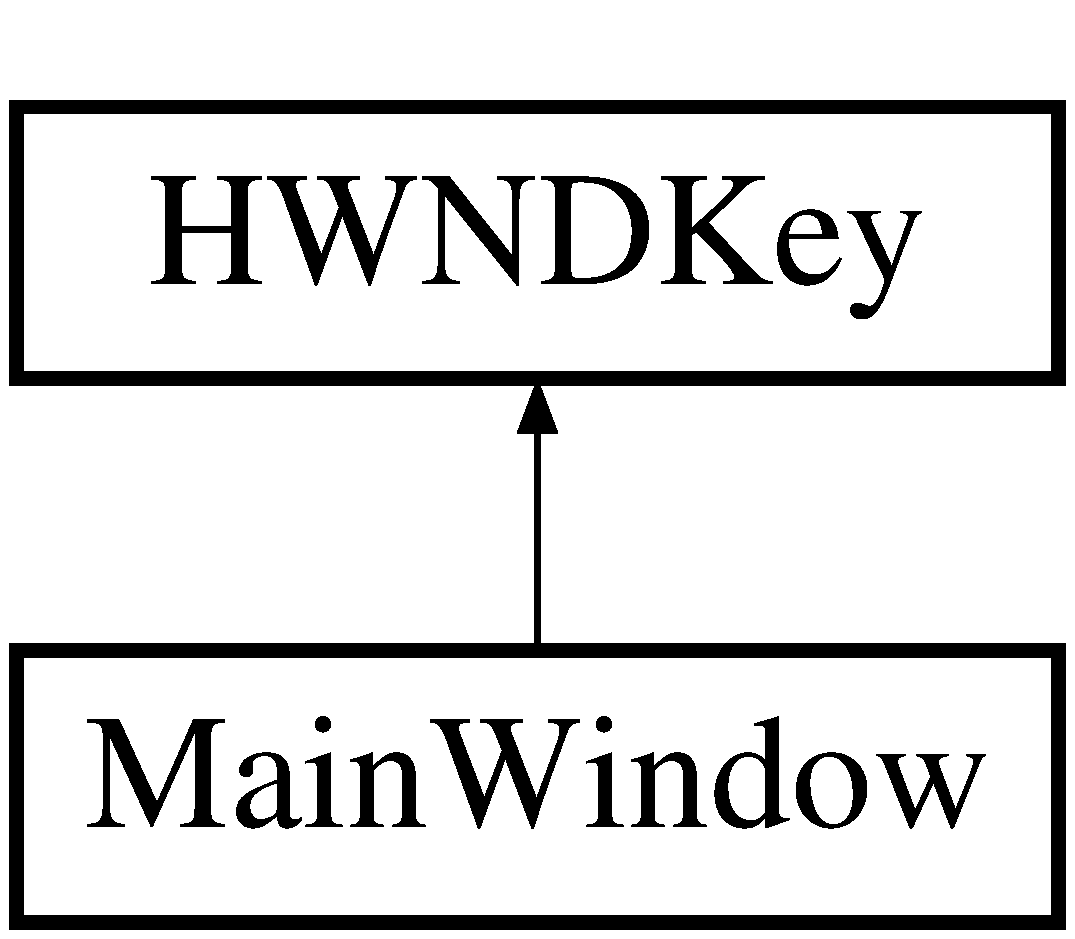
\includegraphics[height=2.000000cm]{class_main_window}
\end{center}
\end{figure}
\subsection*{Classes}
\begin{DoxyCompactItemize}
\item 
class \hyperlink{class_main_window_1_1_exception}{Exception}
\end{DoxyCompactItemize}
\subsection*{Public Member Functions}
\begin{DoxyCompactItemize}
\item 
\mbox{\Hypertarget{class_main_window_a61c12aad464d82e94156c1b1b3e63c7a}\label{class_main_window_a61c12aad464d82e94156c1b1b3e63c7a}} 
{\bfseries Main\+Window} (H\+I\+N\+S\+T\+A\+N\+CE h\+Inst, wchar\+\_\+t $\ast$p\+Args)
\item 
\mbox{\Hypertarget{class_main_window_af1d822d2183a379458e4bc0e2ea2bf3b}\label{class_main_window_af1d822d2183a379458e4bc0e2ea2bf3b}} 
{\bfseries Main\+Window} (const \hyperlink{class_main_window}{Main\+Window} \&)=delete
\item 
\mbox{\Hypertarget{class_main_window_aaa4474cfd4fdb8d3386764a6eb1a4684}\label{class_main_window_aaa4474cfd4fdb8d3386764a6eb1a4684}} 
\hyperlink{class_main_window}{Main\+Window} \& {\bfseries operator=} (const \hyperlink{class_main_window}{Main\+Window} \&)=delete
\item 
\mbox{\Hypertarget{class_main_window_a202e0f89c8b5cb7f4768172f35e49a1b}\label{class_main_window_a202e0f89c8b5cb7f4768172f35e49a1b}} 
bool {\bfseries Is\+Active} () const
\item 
\mbox{\Hypertarget{class_main_window_affb4bb2c05bec8b71998772cfb94b43b}\label{class_main_window_affb4bb2c05bec8b71998772cfb94b43b}} 
bool {\bfseries Is\+Minimized} () const
\item 
\mbox{\Hypertarget{class_main_window_a62dfc452524272c3153ca334c79d16d4}\label{class_main_window_a62dfc452524272c3153ca334c79d16d4}} 
void {\bfseries Show\+Message\+Box} (const std\+::wstring \&title, const std\+::wstring \&message) const
\item 
\mbox{\Hypertarget{class_main_window_a35f292c078d17dcf4b6bc29506c354ec}\label{class_main_window_a35f292c078d17dcf4b6bc29506c354ec}} 
void {\bfseries Kill} ()
\item 
\mbox{\Hypertarget{class_main_window_af0d6ad5abee9b887e41b432d744aa521}\label{class_main_window_af0d6ad5abee9b887e41b432d744aa521}} 
bool {\bfseries Process\+Message} ()
\item 
\mbox{\Hypertarget{class_main_window_aeac01b46a008ab1973df8622edb96e74}\label{class_main_window_aeac01b46a008ab1973df8622edb96e74}} 
const std\+::wstring \& {\bfseries Get\+Args} () const
\end{DoxyCompactItemize}
\subsection*{Public Attributes}
\begin{DoxyCompactItemize}
\item 
\mbox{\Hypertarget{class_main_window_a94fc57f35085d78df196459a5d4bb3a6}\label{class_main_window_a94fc57f35085d78df196459a5d4bb3a6}} 
\hyperlink{class_keyboard}{Keyboard} {\bfseries kbd}
\item 
\mbox{\Hypertarget{class_main_window_a95582efcb4d3547a6069b7fe24aa7d78}\label{class_main_window_a95582efcb4d3547a6069b7fe24aa7d78}} 
\hyperlink{class_mouse}{Mouse} {\bfseries mouse}
\end{DoxyCompactItemize}
\subsection*{Additional Inherited Members}


The documentation for this class was generated from the following files\+:\begin{DoxyCompactItemize}
\item 
Main\+Window.\+h\item 
Main\+Window.\+cpp\end{DoxyCompactItemize}

\hypertarget{class_mouse}{}\section{Mouse Class Reference}
\label{class_mouse}\index{Mouse@{Mouse}}
\subsection*{Classes}
\begin{DoxyCompactItemize}
\item 
class \hyperlink{class_mouse_1_1_event}{Event}
\end{DoxyCompactItemize}
\subsection*{Public Member Functions}
\begin{DoxyCompactItemize}
\item 
\mbox{\Hypertarget{class_mouse_a589f01769018752ebb09b4065892d2ba}\label{class_mouse_a589f01769018752ebb09b4065892d2ba}} 
{\bfseries Mouse} (const \hyperlink{class_mouse}{Mouse} \&)=delete
\item 
\mbox{\Hypertarget{class_mouse_a819e86107c42969fbd14511ce7b30898}\label{class_mouse_a819e86107c42969fbd14511ce7b30898}} 
\hyperlink{class_mouse}{Mouse} \& {\bfseries operator=} (const \hyperlink{class_mouse}{Mouse} \&)=delete
\item 
\mbox{\Hypertarget{class_mouse_abc884bba293fe55e3069b21b7c1d78ac}\label{class_mouse_abc884bba293fe55e3069b21b7c1d78ac}} 
std\+::pair$<$ int, int $>$ {\bfseries Get\+Pos} () const
\item 
\mbox{\Hypertarget{class_mouse_ac80c44d9454043b9f41a636886396e4a}\label{class_mouse_ac80c44d9454043b9f41a636886396e4a}} 
int {\bfseries Get\+PosX} () const
\item 
\mbox{\Hypertarget{class_mouse_ada9ba37672842e0968252ae9dd737891}\label{class_mouse_ada9ba37672842e0968252ae9dd737891}} 
int {\bfseries Get\+PosY} () const
\item 
\mbox{\Hypertarget{class_mouse_a368d450d32e6577d13c49782ca1dd9a7}\label{class_mouse_a368d450d32e6577d13c49782ca1dd9a7}} 
bool {\bfseries Left\+Is\+Pressed} () const
\item 
\mbox{\Hypertarget{class_mouse_afc3a95d7c88453a34ee9747dcd2057b0}\label{class_mouse_afc3a95d7c88453a34ee9747dcd2057b0}} 
bool {\bfseries Right\+Is\+Pressed} () const
\item 
\mbox{\Hypertarget{class_mouse_aac019d97e3890d863b26ed9eff1e3588}\label{class_mouse_aac019d97e3890d863b26ed9eff1e3588}} 
bool {\bfseries Is\+In\+Window} () const
\item 
\mbox{\Hypertarget{class_mouse_a4871a2637c79bfedb316f7f66e939baf}\label{class_mouse_a4871a2637c79bfedb316f7f66e939baf}} 
\hyperlink{class_mouse_1_1_event}{Mouse\+::\+Event} {\bfseries Read} ()
\item 
\mbox{\Hypertarget{class_mouse_ae331dd2ea0826da1e1e0daa081841369}\label{class_mouse_ae331dd2ea0826da1e1e0daa081841369}} 
bool {\bfseries Is\+Empty} () const
\item 
\mbox{\Hypertarget{class_mouse_a240cd0d00a0aa4a57ceafeec058b256d}\label{class_mouse_a240cd0d00a0aa4a57ceafeec058b256d}} 
void {\bfseries Flush} ()
\end{DoxyCompactItemize}
\subsection*{Friends}
\begin{DoxyCompactItemize}
\item 
\mbox{\Hypertarget{class_mouse_af9db4b672c4d3104f5541893e08e1809}\label{class_mouse_af9db4b672c4d3104f5541893e08e1809}} 
class {\bfseries Main\+Window}
\end{DoxyCompactItemize}


The documentation for this class was generated from the following files\+:\begin{DoxyCompactItemize}
\item 
Mouse.\+h\item 
Mouse.\+cpp\end{DoxyCompactItemize}

\hypertarget{class_pixel_location}{}\section{Pixel\+Location Class Reference}
\label{class_pixel_location}\index{Pixel\+Location@{Pixel\+Location}}
\subsection*{Public Member Functions}
\begin{DoxyCompactItemize}
\item 
\mbox{\Hypertarget{class_pixel_location_a4229aa113847e419bb8427bfb37a55cf}\label{class_pixel_location_a4229aa113847e419bb8427bfb37a55cf}} 
{\bfseries Pixel\+Location} (int x, int y)
\item 
\mbox{\Hypertarget{class_pixel_location_aa358ab02675b229e547a5b582d6c2ebf}\label{class_pixel_location_aa358ab02675b229e547a5b582d6c2ebf}} 
void {\bfseries add} (const \hyperlink{class_pixel_location}{Pixel\+Location} \&val)
\end{DoxyCompactItemize}
\subsection*{Public Attributes}
\begin{DoxyCompactItemize}
\item 
\mbox{\Hypertarget{class_pixel_location_ad237ab10b1aa7248dc29b57e45c0de93}\label{class_pixel_location_ad237ab10b1aa7248dc29b57e45c0de93}} 
int {\bfseries x}
\item 
\mbox{\Hypertarget{class_pixel_location_a4dbe2d4b3ee1402f0d06e4d7e577fbd4}\label{class_pixel_location_a4dbe2d4b3ee1402f0d06e4d7e577fbd4}} 
int {\bfseries y}
\end{DoxyCompactItemize}
\subsection*{Friends}
\begin{DoxyCompactItemize}
\item 
\mbox{\Hypertarget{class_pixel_location_aa18747fd0126b0c3aae3a5607d6f0558}\label{class_pixel_location_aa18747fd0126b0c3aae3a5607d6f0558}} 
bool {\bfseries operator==} (const \hyperlink{class_pixel_location}{Pixel\+Location} \&lhs, const \hyperlink{class_pixel_location}{Pixel\+Location} \&rhs)
\end{DoxyCompactItemize}


The documentation for this class was generated from the following files\+:\begin{DoxyCompactItemize}
\item 
Pixel\+Location.\+h\item 
Pixel\+Location.\+cpp\end{DoxyCompactItemize}

\hypertarget{class_snake}{}\section{Snake Class Reference}
\label{class_snake}\index{Snake@{Snake}}
\subsection*{Public Member Functions}
\begin{DoxyCompactItemize}
\item 
\mbox{\Hypertarget{class_snake_a956bd91b03fb8c0bb2a8787ba653cf8d}\label{class_snake_a956bd91b03fb8c0bb2a8787ba653cf8d}} 
void {\bfseries move\+By} (const \hyperlink{class_pixel_location}{Pixel\+Location} \&delta\+Loc, \hyperlink{class_board}{Board} \&brd)
\item 
\mbox{\Hypertarget{class_snake_a959eeb2c461a36a9e51de931d6917a75}\label{class_snake_a959eeb2c461a36a9e51de931d6917a75}} 
void {\bfseries grow} ()
\item 
\mbox{\Hypertarget{class_snake_adc3035ef6074a4cc8467f36836f8fcfc}\label{class_snake_adc3035ef6074a4cc8467f36836f8fcfc}} 
void {\bfseries draw} (\hyperlink{class_board}{Board} \&brd) const
\item 
\mbox{\Hypertarget{class_snake_a71d9b9edb90aab30269a0fae800a325f}\label{class_snake_a71d9b9edb90aab30269a0fae800a325f}} 
bool {\bfseries is\+In\+Location} (const \hyperlink{class_pixel_location}{Pixel\+Location} \&loc) const
\item 
\mbox{\Hypertarget{class_snake_a470d6d5c440ab7b1261977abeddcbb08}\label{class_snake_a470d6d5c440ab7b1261977abeddcbb08}} 
\hyperlink{class_pixel_location}{Pixel\+Location} {\bfseries get\+Next\+Head\+Location} (const \hyperlink{class_pixel_location}{Pixel\+Location} delta\+Loc) const
\end{DoxyCompactItemize}
\subsection*{Static Public Attributes}
\begin{DoxyCompactItemize}
\item 
\mbox{\Hypertarget{class_snake_a53b9c54b0a9f2e07eee5d06b481839f7}\label{class_snake_a53b9c54b0a9f2e07eee5d06b481839f7}} 
static constexpr int {\bfseries M\+O\+V\+E\+\_\+\+P\+E\+R\+I\+OD} = 20
\end{DoxyCompactItemize}


The documentation for this class was generated from the following files\+:\begin{DoxyCompactItemize}
\item 
Snake.\+h\item 
Snake.\+cpp\end{DoxyCompactItemize}

\hypertarget{class_sprite_codex}{}\section{Sprite\+Codex Class Reference}
\label{class_sprite_codex}\index{Sprite\+Codex@{Sprite\+Codex}}
\subsection*{Static Public Member Functions}
\begin{DoxyCompactItemize}
\item 
\mbox{\Hypertarget{class_sprite_codex_ab54c26dad73c7af8ed9710882b00fcff}\label{class_sprite_codex_ab54c26dad73c7af8ed9710882b00fcff}} 
static void {\bfseries Draw\+Game\+Over} (int x, int y, \hyperlink{class_graphics}{Graphics} \&gfx)
\item 
\mbox{\Hypertarget{class_sprite_codex_a0ec729dc12ae0f15800415f6bb54e29b}\label{class_sprite_codex_a0ec729dc12ae0f15800415f6bb54e29b}} 
static void {\bfseries Draw\+Title} (int x, int y, \hyperlink{class_graphics}{Graphics} \&gfx)
\end{DoxyCompactItemize}


The documentation for this class was generated from the following files\+:\begin{DoxyCompactItemize}
\item 
Sprite\+Codex.\+h\item 
Sprite\+Codex.\+cpp\end{DoxyCompactItemize}

%--- End generated contents ---

% Index
\backmatter
\newpage
\phantomsection
\clearemptydoublepage
\addcontentsline{toc}{chapter}{Index}
\printindex

\end{document}
